\section{Prototipo (Aplicaci�n)}
\begin{frame}%[allowframebreaks]
	\frametitle{Prototipo (Aplicaci�n)}

	\begin{block}
	\justifying 
	\small Una aplicaci�n Web para que los usuarios puedan consultar y visualizar la informaci�n de los \textit{recursos de informaci�n}, proveniente de un modelo sem�ntico.
	\end{block}
\end{frame}

\begin{frame}%[allowframebreaks]
	\frametitle{Navegaci�n entre informaci�n de los recursos de informaci�n}
	\begin{figure}
	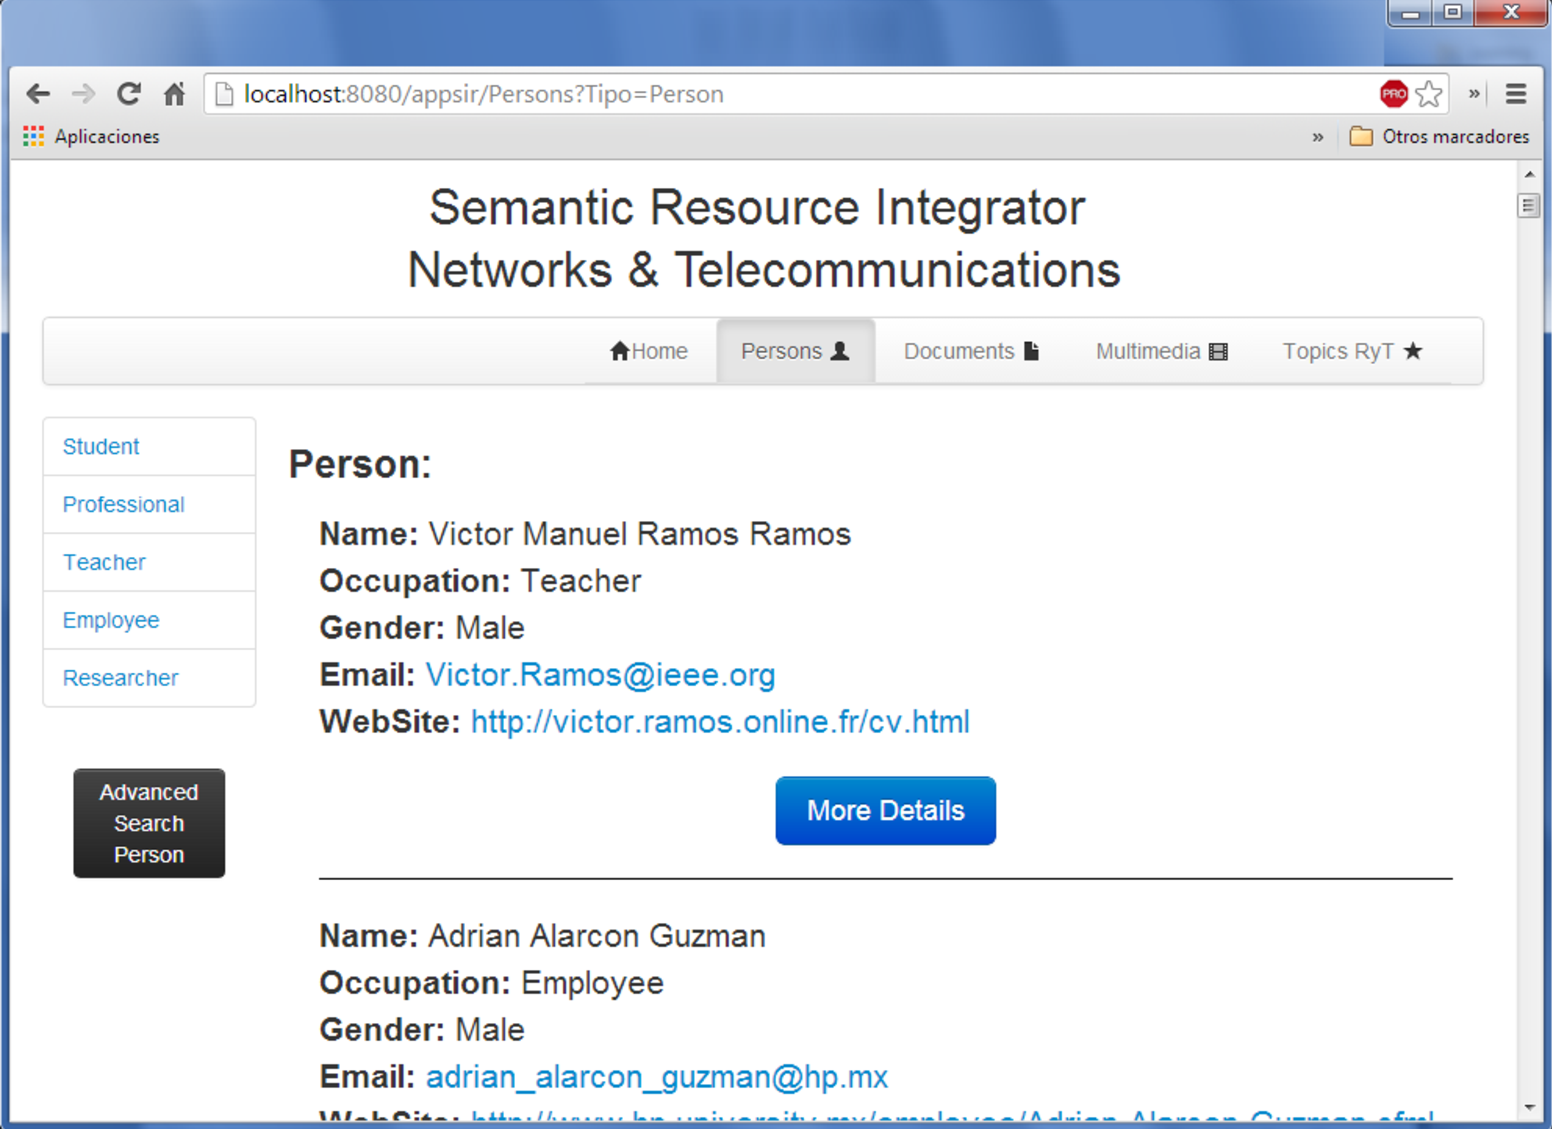
\includegraphics[scale=0.35]{IntWebNavPer} 
	\end{figure}
\end{frame}

\begin{frame}%[allowframebreaks]
	\frametitle{B�squeda Avanzada de los recursos de informaci�n}
	\begin{figure}
	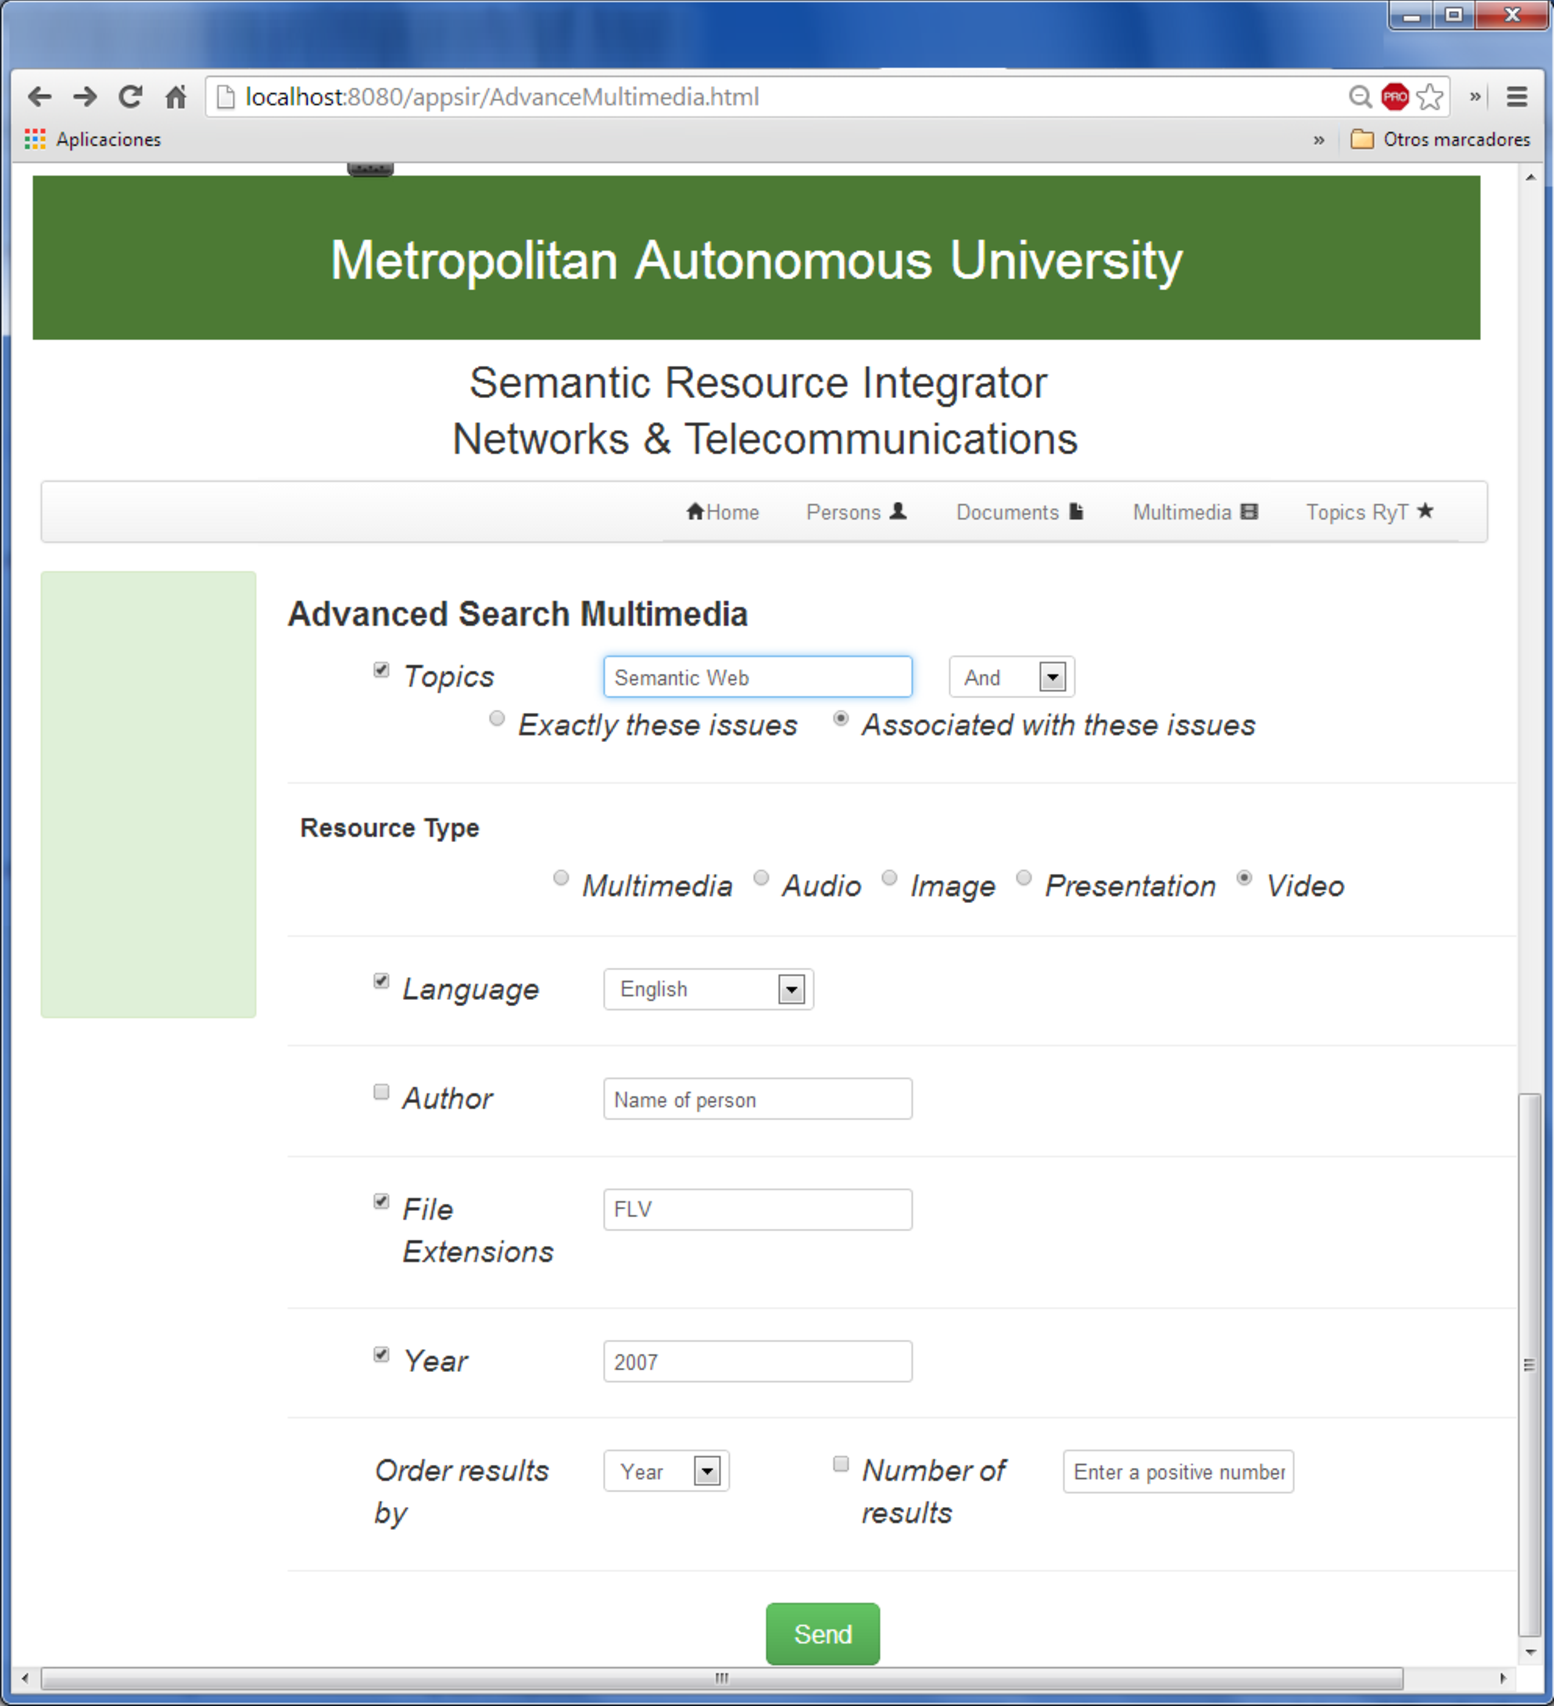
\includegraphics[scale=0.23]{FormBusMult} 
	\end{figure}
\end{frame}

%\begin{frame}%[allowframebreaks]
%	\frametitle{Detalles de un recurso de informaci�n}
%	\begin{figure}
%	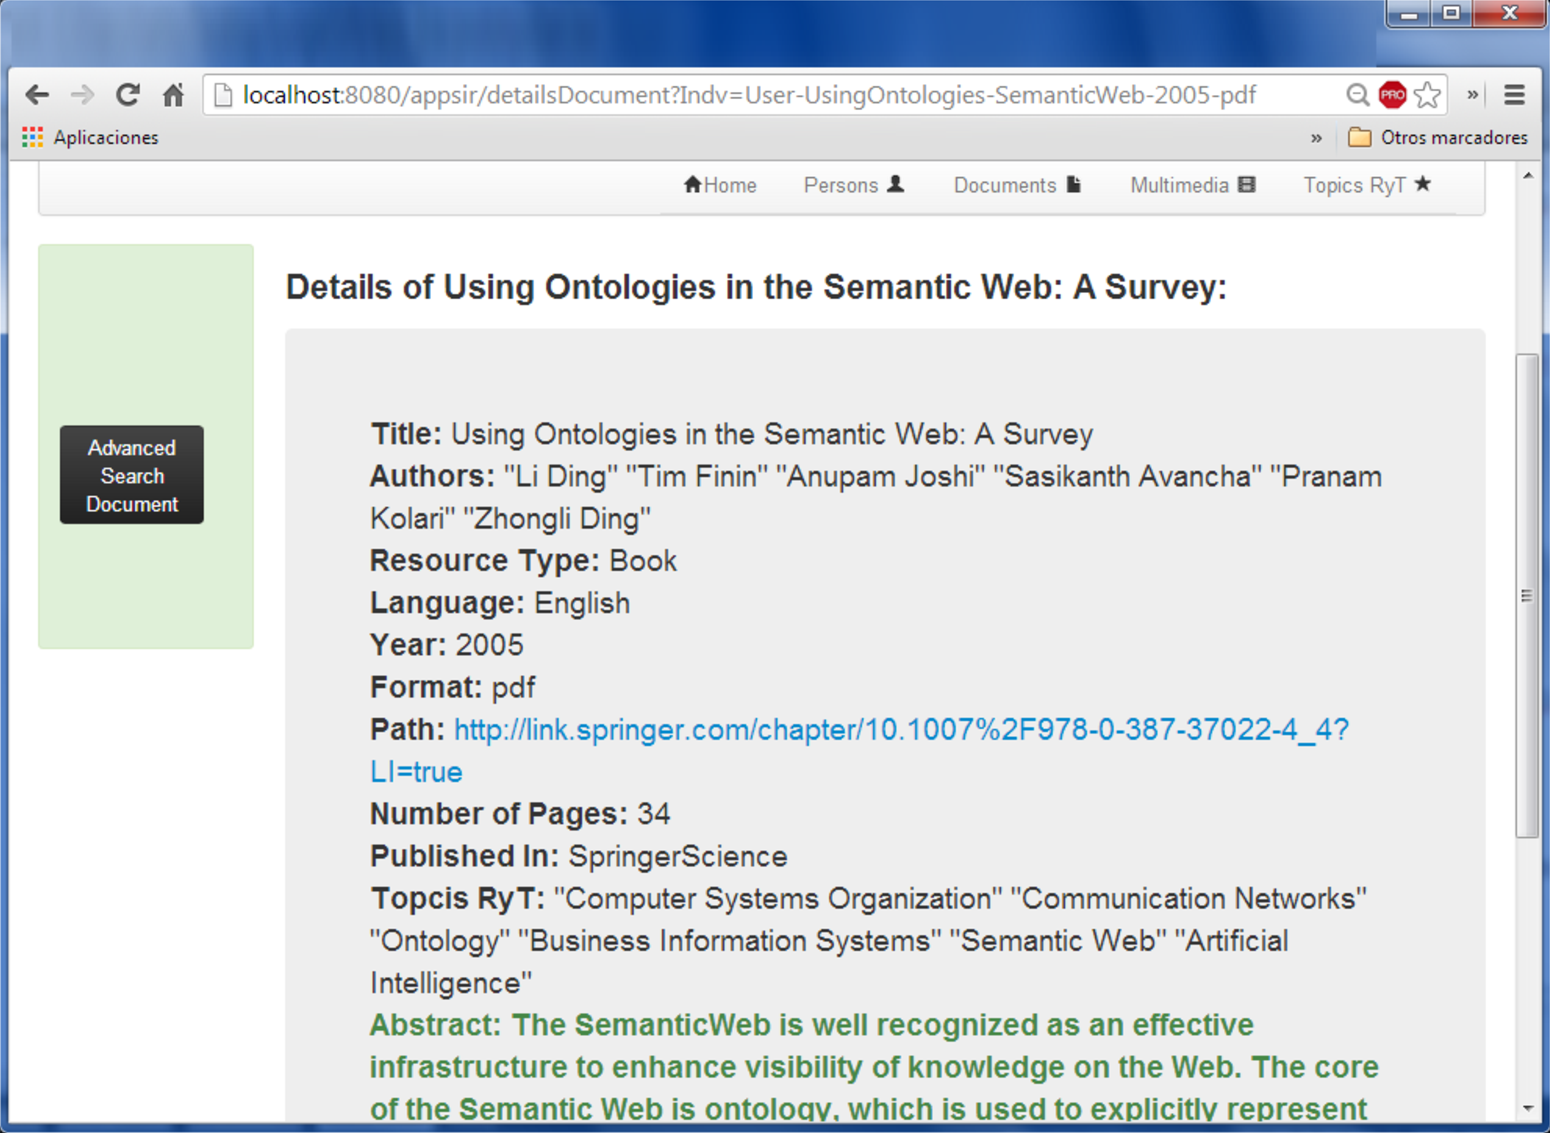
\includegraphics[scale=0.35]{IntWebDetDoc} 
%	\end{figure}
%\end{frame}